\documentclass[12pt]{article}
%%---------------------------------------------------------------------
% packages
% geometry
\usepackage{geometry}
% font
\usepackage{fontspec}
\defaultfontfeatures{Mapping=tex-text}  %%如果没有它,会有一些 tex 特殊字符无法正常使用,比如连字符。
\usepackage{xunicode,xltxtra}
\usepackage[BoldFont,SlantFont,CJKnumber,CJKchecksingle]{xeCJK}  % \CJKnumber{12345}: 一万二千三百四十五
\usepackage{CJKfntef}  %%实现对汉字加点、下划线等。
\usepackage{pifont}  % \ding{}
% math
\usepackage{amsmath,amsfonts,amssymb}
% color
\usepackage{color}
\usepackage{xcolor}
\definecolor{EYE}{RGB}{199,237,204}
\definecolor{FLY}{RGB}{128,0,128}
\definecolor{ZHY}{RGB}{139,0,255}
% graphics
\usepackage[americaninductors,europeanresistors]{circuitikz}
\usepackage{tikz}
\usetikzlibrary{positioning,arrows,shadows,shapes,calc,mindmap,trees,backgrounds}  % placements=positioning
\usepackage{graphicx}  % \includegraphics[]{}
\usepackage{subfigure}  %%图形或表格并排排列
% table
\usepackage{colortbl,dcolumn}  %% 彩色表格
\usepackage{multirow}
\usepackage{multicol}
\usepackage{booktabs}
% code
\usepackage{fancyvrb}
\usepackage{listings}
% title
\usepackage{titlesec}
% head/foot
\usepackage{fancyhdr}
% ref
\usepackage{hyperref}
% pagecolor
\usepackage[pagecolor={EYE}]{pagecolor}
% tightly-packed lists
\usepackage{mdwlist}

\usepackage{styles/iplouccfg}
\usepackage{styles/zhfontcfg}
\usepackage{styles/iplouclistings}

%%---------------------------------------------------------------------
% settings
% geometry
\geometry{left=2cm,right=1cm,top=2cm,bottom=2cm}  %设置 上、左、下、右 页边距
\linespread{1.5} %行间距
% font
\setCJKmainfont{Adobe Kaiti Std}
%\setmainfont[BoldFont=Adobe Garamond Pro Bold]{Apple Garamond}  % 英文字体
%\setmainfont[BoldFont=Adobe Garamond Pro Bold,SmallCapsFont=Apple Garamond,SmallCapsFeatures={Scale=0.7}]{Apple Garamond}  %%苹果字体没有SmallCaps
\setCJKmonofont{Adobe Fangsong Std}
% graphics
\graphicspath{{figures/}}
\tikzset{
    % Define standard arrow tip
    >=stealth',
    % Define style for boxes
    punkt/.style={
           rectangle,
           rounded corners,
           draw=black, very thick,
           text width=6.5em,
           minimum height=2em,
           text centered},
    % Define arrow style
    pil/.style={
           ->,
           thick,
           shorten <=2pt,
           shorten >=2pt,},
    % Define style for FlyZhyBall
    FlyZhyBall/.style={
      circle,
      minimum size=6mm,
      inner sep=0.5pt,
      ball color=red!50!blue,
      text=white,},
    % Define style for FlyZhyRectangle
    FlyZhyRectangle/.style={
      rectangle,
      rounded corners,
      minimum size=6mm,
      ball color=red!50!blue,
      text=white,},
    % Define style for zhyfly
    zhyfly/.style={
      rectangle,
      rounded corners,
      minimum size=6mm,
      ball color=red!25!blue,
      text=white,},
    % Define style for new rectangle
    nrectangle/.style={
      rectangle,
      draw=#1!50,
      fill=#1!20,
      minimum size=5mm,
      inner sep=0.1pt,}
}
\ctikzset{
  bipoles/length=.8cm
}
% code
\lstnewenvironment{VHDLcode}[1][]{%
  \lstset{
    basicstyle=\footnotesize\ttfamily\color{black},%
    columns=flexible,%
    framexleftmargin=.7mm,frame=shadowbox,%
    rulesepcolor=\color{blue},%
%    frame=single,%
    backgroundcolor=\color{yellow!20},%
    xleftmargin=1.2\fboxsep,%
    xrightmargin=.7\fboxsep,%
    numbers=left,numberstyle=\tiny\color{blue},%
    numberblanklines=false,numbersep=7pt,%
    language=VHDL%
    }\lstset{#1}}{}
\lstnewenvironment{VHDLmiddle}[1][]{%
  \lstset{
    basicstyle=\scriptsize\ttfamily\color{black},%
    columns=flexible,%
    framexleftmargin=.7mm,frame=shadowbox,%
    rulesepcolor=\color{blue},%
%    frame=single,%
    backgroundcolor=\color{yellow!20},%
    xleftmargin=1.2\fboxsep,%
    xrightmargin=.7\fboxsep,%
    numbers=left,numberstyle=\tiny\color{blue},%
    numberblanklines=false,numbersep=7pt,%
    language=VHDL%
    }\lstset{#1}}{}
\lstnewenvironment{VHDLsmall}[1][]{%
  \lstset{
    basicstyle=\tiny\ttfamily\color{black},%
    columns=flexible,%
    framexleftmargin=.7mm,frame=shadowbox,%
    rulesepcolor=\color{blue},%
%    frame=single,%
    backgroundcolor=\color{yellow!20},%
    xleftmargin=1.2\fboxsep,%
    xrightmargin=.7\fboxsep,%
    numbers=left,numberstyle=\tiny\color{blue},%
    numberblanklines=false,numbersep=7pt,%
    language=VHDL%
    }\lstset{#1}}{}
% pdf
\hypersetup{pdfpagemode=FullScreen,%
            pdfauthor={Haiyong Zheng},%
            pdftitle={Title},%
            CJKbookmarks=true,%
            bookmarksnumbered=true,%
            bookmarksopen=false,%
            plainpages=false,%
            colorlinks=true,%
            citecolor=green,%
            filecolor=magenta,%
            linkcolor=cyan,%red(default)
            urlcolor=cyan}
% section
%http://tex.stackexchange.com/questions/34288/how-to-place-a-shaded-box-around-a-section-label-and-name
\newcommand\titlebar{%
\tikz[baseline,trim left=3.1cm,trim right=3cm] {
    \fill [cyan!25] (2.5cm,-1ex) rectangle (\textwidth+3.1cm,2.5ex);
    \node [
        fill=cyan!60!white,
        anchor= base east,
        rounded rectangle,
        minimum height=3.5ex] at (3cm,0) {
        \textbf{\thesection.}
    };
}%
}
\titleformat{\section}{\Large\bf\color{blue}}{\titlebar}{0.1cm}{}
% head/foot
\setlength{\headheight}{15pt}
\pagestyle{fancy}
\fancyhf{}
%\lhead{\color{black!50!green}2014年秋季学期}
\chead{\color{black!50!green}图像特征}
%\rhead{\color{black!50!green}通信电子电路}
\lfoot{\color{blue!50!green}朱亚菲}
\cfoot{\color{blue!50!green}\href{http://vision.ouc.edu.cn/~zhenghaiyong}{CVBIOUC}}
\rfoot{\color{blue!50!green}$\cdot$\ \thepage\ $\cdot$}
\renewcommand{\headrulewidth}{0.4pt}
\renewcommand{\footrulewidth}{0.4pt}


%%---------------------------------------------------------------------
\begin{document}
%%---------------------------------------------------------------------
%%---------------------------------------------------------------------
% \titlepage
\title{\vspace{-2em}显著性检测领域之图像特征\vspace{-0.7em}}
\author{朱亚菲}
\date{\vspace{-0.7em}2015年1月\vspace{-0.7em}}
%%---------------------------------------------------------------------
\maketitle\thispagestyle{fancy}
%%---------------------------------------------------------------------
\maketitle
\tableofcontents 


\section{引言}

图像特征提取是图像分析与图像识别的前提,它是将高维的图像数据进行简化表达最有效的方式,从一幅图像的$M \times N \times3$的数据矩阵中,我们看不出任何信息,所以我们必须根据这些数据提取出图像中的关键信息,一些基本元件以及它们的关系。

图像特征可分为全局特征和局部特征。其最大的区别是特征提取的空间范围不同。全局特征是从整个图像中提取的特征,而局部特征是从图像区域中提取的特征。全局特征容易受到环境的干扰,光照、旋转、噪声等不利因素都会影响全局特征。相比而言,局部特征点,往往对应着图像中的一些线条交叉、明暗变化的结构中,受到的干扰也少。

总的来说,全局特征是对图像内容的高度抽象的概括。如果用户对整个图像的整体感兴趣,而不是对前景本身感兴趣的话,用全局特征来描述图像是比较合适的。但是无法分辨出前景和背景却是全局特征本身就有的劣势,特别是在关注的对象受到遮挡等影响的时候,全局特征很有可能就被破坏掉了。

在显著性检测中,由于关注的是显著目标,并且是在同一幅图像中进行中央-周围/局部/全局对比,而不是在图像间进行比较,因此用到的应该都是局部特征。显著性检测领域所说的局部和全局方法是指对某一像素或区域,在计算其对比度时是与周围相比还是与图像中所有其它像素或区域相比。

基于像素级或block级的显著性检测方法中用到是center-surround contrast或global contrast,而基于区域的方法用到的则是local contrast或global contrast,这是因为区域形状不规则,所以叫local contrast。

英国Oxford大学的Andrea Valida,他是VLFeat的发起者和主要作者。VLFeat官方主页:\url{vlfeat.org}。它一个实现了计算机视觉领域诸多算法的开源库,包括SIFT,HOG等等。底层代码用C语言实现,并提供了MATLAB接口。支持Windows,Mac OS X和Linux。VLFeat目前正在逐渐实现其他常用的特征描述子。和OpenCV相比,VLFeat是一个轻量级的库,主要实现了在特征提取和聚类方面的高效算法,可以用在图像检索和物体识别领域中。

\url{http://www.sigvc.org/bbs/thread-165-1-1.html}

图像特征又可以分为低层次特征和高层次特征。其中低层次特征是不需要任何形状信息(空间关系的信息)就可以从图像中自动提取的基本特征。高层次特征提取关心的是在图像中找出形状。例如,要自动识别人脸,一种方法是提取组成部分特征。也就是说,需要提取眼睛、耳朵和鼻子这些主要的脸部特征。这些特征可以利用它们的形状找到:眼睛的白色部分是椭圆形的;嘴巴可以看做是两条直线,眉毛也一样。形状提取意味着找出它们的位置、朝向和尺寸。所有低层次方法都可以应用于高层次特征提取,从而在图像中找到形状。

\section{基于像素点的feature contrasts}

\subsection{颜色特征}

\subsubsection{彩色模型}

彩色模型(也称为彩色空间或彩色系统)的目的是在某些标准下用通常可以接受的方式方便地对彩色加以说明。

1)RGB颜色模型

RGB颜色空间是常用的表示彩色图像的一种颜色空间,它是以红、绿、蓝三种颜色为基础,亦称为“三原色”。所谓的“原色”是一种生物学概念,是根据人眼对光线感知的生理作用来定义的。每一种颜色按亮度进行分类,分成256个等级。不同比例的红、绿、蓝叠加,能产生丰富的颜色。例如,等比例的三原色进行相加可以产生白色,红色与绿色相加产生黄色。可见,RGB空间属于“叠加型”原色系统,因此把RGB颜色空间作为最基础的颜色空间,通过对RGB的非线性或线性变换可以获得其它的颜色空间。

2)CIELAB颜色空间

在许多文献中,CIELAB颜色空间也称CIE 1976 L*a*b(简写为CIE L*a*b)颜色空间。CIELAB颜色系统是使用最广泛的物体颜色度量方法,并作为度量颜色的国际标准。CIE 1976 L*a*b颜色空间是CIE 1931 XYZ颜色空间的一种数学变换的结果。

CIE 1976 L*a*b颜色空间和CIE 1931 XYZ颜色空间的相同之处是,它们都使用相同的基本原理,即颜色是光、物体和观察者组合的结果,三种基色值是用CIE定义的光、物体和观察者的数据进行计算得到的。

CIELAB系统使用的坐标叫做对色坐标(opponent color coordinate),使用对色坐标的想法来自这样的概念:颜色不能同时是红和绿,或者同时是黄和蓝,但颜色可以被认为是红和黄、红和蓝、绿和黄以及绿和蓝的组合。CIELAB使用L*, a*和b*坐标轴定义CIE颜色空间。其中,L*值代表光亮度,其值从0(黑色)~100(白色)。a*和b*代表色度坐标,其中a*代表红-绿轴,b*代表黄-蓝轴,它们的值从0~10。$a*=b*=0$表示无色,因此L*就代表从黑到白的比例系数。

\subsection{SIFT特征}

SIFT特征(Scale-invariant transform,尺度不变特征变换)由David Lowe在1999年~\cite{lowe1999object}所发表,2004年~\cite{lowe2004distinctive}完善总结。它是一种计算机视觉的算法,用来侦测与描述图像中的局部性特征,它在空间尺度中寻找极值点,并提取出其位置、尺度、旋转不变量。SIFT算法提取的特征点具有尺度不变性,也就是说,同一物体在图像上不论尺度大小,都能根据SIFT算法提取到相同的特征点。

简单来说,SIFT算法就是用不同尺度(标准差)的高斯函数对图像进行平滑,然后比较平滑后图像的差别,差别大的像素就是特征明显的点。

尺度空间理论的目的是模拟图像数据的多尺度特征。高斯卷积核是实现尺度变换的唯一线性核,于是一幅二维图像的尺度空间定义为:
\begin{align}
L(x, y, e) = G(x, y, e) * I(x, y)
\end{align}

其中$G(x, y, e$是尺度可变高斯函数,
\begin{align}
 G(x,y,e) = \frac{1}{2*\pi *e^2} * exp[-\frac{x^2 + y^2}{2e^2}]
\end{align}

$(x, y)$是空间坐标,$e$是尺度坐标。

为了有效地在尺度空间检测到稳定的关键点,提出了高斯差分尺度空间(DOG scale-space)。利用不同尺度的高斯差分核与图像卷积生成。
\begin{align}
D(x,y,e) = ((G(x,y,ke) - G(x,y,e)) * I(x,y) = L(x,y,ke) - L(x,y,e)
\end{align}

SIFT特征一般用于匹配,在eye fixation prediction中有用到,而在显著性区域检测中没有见用的。

\section{基于区域的feature contrasts}

这里的feature contrasts是指由某种visual cue(比如颜色、纹理、位置等)对图像中两个区域$r_i$、$r_j$求出的区域间对比度。

\subsection{颜色}

\subsubsection{Color Contrast}

论文~\cite{yan2013hierarchical}中用到,公式如下:
\begin{align}
C_i = \sum_{j=1}^{n}w(R_i)\Phi(i, j)||c_i-c_j||_2
\end{align}
其中,$c_i$和$c_j$分别是区域$R_i$和$R_j$内颜色的均值,$w(R_j)$表示区域$R_j$内的像素个数,$\Phi(i, j) = exp\{ -D(R_i, R_j)/\sigma^2\}$。

论文~\cite{zhu2014tag}中用到,图像区域中方差不同的颜色之间的分布是相互独立的。区域$r_i$与$r_j$之间的color contrast定义如下:
\begin{align}
D_c(r_i, r_j) = ||\mu_{c, i}-\mu_{c, j}||^2\cdot \left(\frac{\sigma_{c, i}^2}{n_i}+\frac{\sigma_{c, j}^2}{n_j}\right)^{-\frac{1}{2}}
\end{align}
其中$\mu_{c, i}$和$\mu_{c, j}$分别表示区域$r_i$和$r_j$内的颜色均值,$\sigma_{c, i}^2$和$\sigma_{c, j}^2$表示方差,$n_i$和$n_j$表示相应区域内像素的个数。

\subsubsection{颜色直方图}

图像直方图是指统计图像中像素的灰度/颜色得到的图像灰度/颜色频数图。直方图由于其计算代价较小,且具有图像平移、旋转、缩放不变性等优点,广泛应用于图像处理的各个领域。Swain和Ballard最先提出了使用颜色直方图作为图像颜色特征的表示方法。

传统颜色直方图描述方法存在以下问题:

1)颜色特征维数高。以8bit的RGB颜色空间为例,全颜色数为$256 \times 256 \times 256$种颜色,如果以全颜色数统计直方图,则存储空间和计算复杂度都较大。

2)颜色特征受光照影响。即对于两幅颜色分布很类似却因光照不同导致亮度差异大的图像,理论上,其颜色直方图应相似,但实际传统颜色直方图却不相似。

3)不能表达相近颜色间相关性,即传统颜色直方图的颜色间完全独立,不能反映相近颜色间的关联。理论上,对于发生较小颜色偏移的两幅图像间应相似。如,一幅完全红色的图像与另一幅完全浅红色的图像间相似度较高。而实际传统颜色直方图却不相似。

4)丢失空间位置信息,因此该特征无法区分颜色相同而空间分布不同的两幅图像。

得到图像颜色特征后 需要定义颜色特征的相似度量公式,以表示两幅图像间颜色的相似性。不同的相似性度量公式对实际应用结果可能影响很大。因此需要研究如何选择或设计合适的相似性度量算法。

显著性Models中,CB~\cite{jiang2011automatic}、DRFI~\cite{jiang2013salient}、HC/RC~\cite{cheng2011global}、HDCT~\cite{kim2014salient}方法都用到了颜色直方图。

DRFI方法中关于图像RGB空间的颜色直方图代码如下:

\lstinputlisting{RGBhistogram.m}

首先对图像($300 \times 400$)的颜色空间进行量化,将颜色空间划分为若干个小的颜色区间,即直方图的bin,例如将每个颜色通道量化为只有16个不同值,此时$bin = 16 \times 16 \times 16$,然后计算矩阵$Q$($300 \times 400$),用其中的值代表颜色,而不是用$(r, g, b)$向量表示颜色,$Q$中有多少个不同值表示图像中有多少种颜色。结果如图~\ref{fig: RGBhistogram}。

\begin{figure}
  \centering 
  \subfigure[]{ 
    \label{fig: RGBhistogram: a} %% label for first subfigure 
    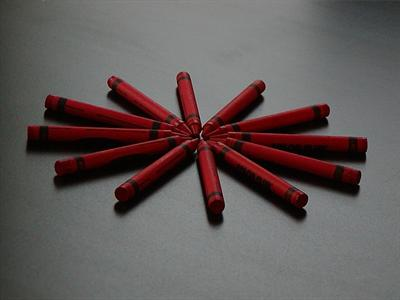
\includegraphics[width=0.45\textwidth]{example1.jpg}} 
  \subfigure[]{ 
    \label{fig: RGBhistogram: b} %% label for second subfigure 
    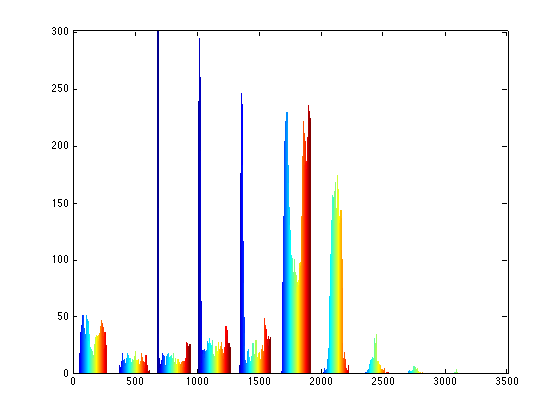
\includegraphics[width=0.45\textwidth]{RGBhistogram1.png}} 
  \caption{RGB空间的颜色直方图}
  \label{fig: RGBhistogram} %% label for entire figure 
\end{figure}

对每个超像素区域,可以知道其中像素点的坐标值,能求出其对应到矩阵$Q$中的值,有多少个不同值就代表该区域内有多少种不同的颜色,然后算该区域在$1-16^3$之间的颜色占的像素个数,没有的记为0。对每个区域都能算出这样一个$16^3$维的向量,然后求区域之间的直方图的对比度,也就是求这样两个向量之间的距离。

\subsection{纹理特征}

图像纹理一直到现在都没有一个一致的、公认的定义,它在图像中是一个重要但是又不太容易描述出来的特征。纹理是人们将人类的视觉与触觉联系起来,进而形成一个视觉信息,它起源于人类对事物的触感。

LBP(Local Binary Pattern,局部二值模式)首先是由Ojala等人~\cite{ojala1994performance}于1994年提出,DRFI方法~\cite{jiang2013salient}中用到。

LBP有很多变种,或说改进。原始的LBP记录像素点与其周围像素点的对比信息,或说差异。对于图像上9个方格中中间方格(方格中的值是像素点灰度值大小),做一个阈值化处理。大于等于中心点像素的,标记为1,小于的则标记为0。最后将中心像素点周围的11110001二进制数化为十进制数,得到LBP值。如图~\ref{fig: LBP}所示。

\begin{figure}[!ht]
\centering
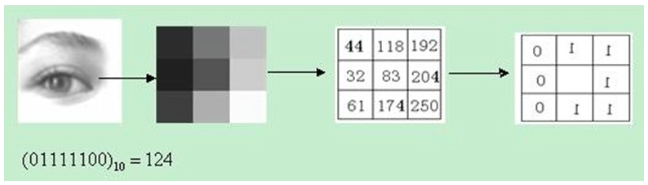
\includegraphics[width=0.6\textwidth]{LBP.png}
\caption{原始LBP}
\label{fig: LBP}
\end{figure} 

如图~\ref{fig: LBP特征}

\begin{figure}
  \centering 
  \subfigure[]{ 
    \label{fig: LBP: a} %% label for first subfigure 
    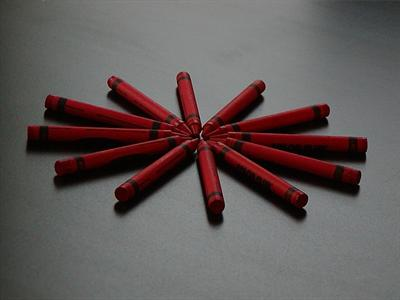
\includegraphics[width=0.45\textwidth]{example1.jpg}} 
  \subfigure[]{ 
    \label{fig: LBP: b} %% label for second subfigure 
    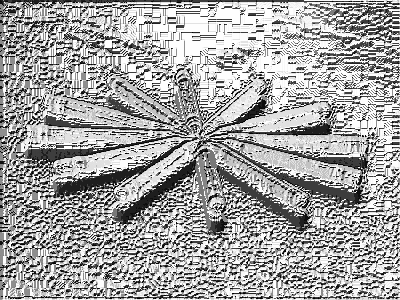
\includegraphics[width=0.45\textwidth]{LBP1.png}} 
  \caption{LBP}
  \label{fig: LBP特征} %% label for entire figure 
\end{figure}

\subsection{位置特征}

超像素区域中心与图像中心的距离

论文~\cite{yan2013hierarchical}中用到,公式如下:
\begin{align}
H_i = \frac{1}{w(R_i)}\sum_{x_i \in R_i} exp\{-\lambda||x_i-x_c||^2\}
\end{align}

其中$(x_0, x_1 \ldots)$是区域$R_i$中的像素坐标集,$x_c$是图像中心的坐标,$w(R_i)$计算了区域$R_i$内的像素个数。由$H_i$的公式可看到,距离图像中心越近的区域拥有越大的权值。

HDCT~\cite{kim2014salient}中用到,

\subsection{形状特征}

\subsubsection{区域面积}

该区域包含的超像素的个数

\subsubsection{奇异值特征}

奇异值特征(Singular Value Feature,SVF)~\cite{su2011blurred}被用来从测试图像中检测模糊区域,通常一幅图像中的模糊区域是背景的可能性较大。

\subsubsection{HOG特征}

HOG(Histogram of Oriented Gradients,方向梯度直方图)特征最早是由法国国家计算机技术和控制研究所(INRIA)的Navneet Dalal和Bill Triggs在2005年发表在CVPR上的论文~\cite{dalal2005histograms}中提出的。

Dalal提出的HOG特征提取的过程如图~\ref{fig: HOG},进一步表述如下:

\begin{figure}[!ht]
\centering
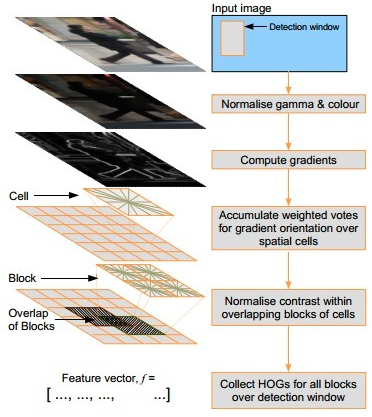
\includegraphics[width=0.6\textwidth]{HOG.png}
\caption{算法流程图}
\label{fig: HOG}
\end{figure} 

1. 灰度化

2. 采用Gamma校正法对输入图像进行颜色空间的标准化(归一化);目的是调节图像的对比度,降低图像局部的阴影和光照变化所造成的影响,同时可以抑制噪音的干扰。Gamma压缩公式:
\begin{align}
I(x, y) = I(x, y)^{gamma}
\end{align}

3. 计算图像每个像素的梯度(包括大小和方向),主要是为了捕获轮廓信息,同时进一步弱化光照的干扰。

图像中像素点$(x, y)$的梯度为
\begin{align}
G_x(x, y) = H(x+1, y) - H(x-1, y) \\
G_y(x, y) = H(x, y+1) - H(x, y-1)
\end{align}

式中$G_x(x, y), G_y(x, y), H(x, y)$分别表示输入图像中像素点$(x, y)$处的水平方向梯度、垂直方向梯度和灰度值。像素点$(x, y)$处的梯度幅值和梯度方向分别为:
\begin{align}
G(x, y) & = \sqrt{G_x(x, y)^2 + G_y(x, y)^2}\\
\alpha(x, y) & = tan^{-1}(\frac{G_y(x, y)}{G_x(x, y)}
\end{align}

最常用的方法是:首先用$[-1, 0, 1]$梯度算子对原图像做卷积运算,得到$x$方向(水平方向,以向右为正方向)的梯度分量gradscalx,然后用$[1, 0, -1]^T$梯度算子对原图像做卷积运算,得到$y$方向(竖直方向,以向上为正方向)的梯度分量gradscaly。然后再用以上公式计算该像素点的梯度大小和方向。

4. 将图像每$16*16$(取其它也可以)个像素分到一个cell中,对于$256*256$的图像来说,就分成了$16*16$个cell了。

5. 对于每个cell求其梯度方向直方图,通常取$bin = 9$(取其它也可以)个方向(特征),也就是每$360/9 = 40$度分到一个方向,形成每个cell的descriptor。如图~\ref{fig: 方向梯度},当某像素的梯度方向是20-40度,然后它的梯度大小是$|grad|$,那么直方图第2
个bin的计数就要加上$|grad|$。

\begin{figure}[!ht]
\centering
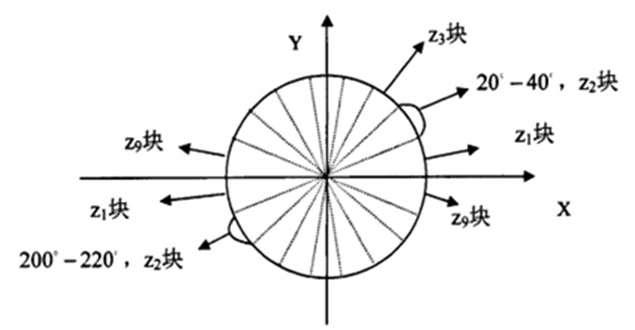
\includegraphics[width=0.5\textwidth]{方向梯度.png}
\caption{梯度方向bin的划分}
\label{fig: 方向梯度}
\end{figure} 

6. 由于局部光照的变化以及前景-背景对比度的变化,使得梯度强度的变化范围非常大。这就需要对梯度强度做归一化。归一化能够进一步地对光照、阴影和边缘进行压缩。为此可以将每$2*2$(取其它也可以)个cell合成一个大的、空间上连通的block,所以这里就有$(16-1)*(16-1) = 225$个block。一个block内所有cell的特征向量串联起来便得到该block的HOG特征。这些block是互有重叠的,这就意味着:每一个cell的特征会以不同的结果多次出现在最后的特征向量中。

7. 所以每个block中都有$2*2*9$个特征,一共有225个block,所以总的特征有$225*36$个。

遇到的疑问:

1)在显著性检测中,先将图像分割成区域,然后怎么提取该区域的HOG特征?

2)一定要将彩色图像先转化为灰度图像才能提取HOG特征吗?

HDCT~\cite{kim2014salient}方法中用到HOG特征~\cite{felzenszwalb2010object},采用的是VLFeat官网上的代码。论文中首先也是对图像进行超像素分割,然后求每个超像素区域内像素点坐标的平均值$(x_i, y_i)$,$i$代表第$i$个超像素区域,求该区域的HOG特征就是以该坐标点为中心的$17*17$的网格作为输入图像(只取该网格内图像r通道的值),17作为cellSize,然后对每个超像素区域得到一个31维的HOG特征向量。


\subsection{Visual Complexity Contrast}

论文~\cite{zhu2014tag}中用到,信息论中可以用熵来计算visual complexity,区域$r_i$和$r_j$之间的visual complexity contrast $D_e(r_i, r_j)$就被定义为
\begin{align}
D_e(r_i, r_j) = [H(r_i)-H(r_j)]^2
\end{align}
其中,$H(r_i)$表示区域$r_i$内的熵
\begin{align}
H(r_i) = \sum_{p=1}^{n_{c, i}}f(c_{p, i})\cdot log_2f(c_{p, i})
\end{align}
其中,$c_{p, i}$是区域$r_i$中第$p$种颜色,$n_{c, i}$区域$r_i$中包含的颜色个数,$f(c_{p, i})$表示区域$r_i$中颜色$c_{p, i}$出现的概率。

\subsection{Background Weighted Contrast}

论文~\cite{zhu2014saliency}中用到

\section{Feature Contrasts的融合}

目前来看,分为两种。

1. 求出两个区域间关于多种关于visual cues的对比度之后,要先将这些对比度融合,例如可以相乘,求出最终的对比度公式。然后再对每个区域计算local或global contrast。

论文~\cite{zhu2014tag}中,两个区域$r_i$、$r_j$间的最终的对比度定义如下:
\begin{align}
D_r(r_i, r_j) = D_c(r_i, r_j) \cdot exp[\sigma_e^2 \cdot D_e(r_i, r_j)]
\end{align}
其中$D_c(r_i, r_j)$是指color contrast,$D_c(r_i, r_j)$是指visual complexity contrast。

对每个区域$r_i$,其空间加权global contrast定义为:
\begin{align}
U(r_i) = \sum_{j\ne i}w_{ij} \cdot D_r(r_i, r_j) \cdot \phi_j\\
w_{ij} = \frac{1}{Z_i}\cdot exp[-\sigma_s^2 \cdot D_s(r_i, r_j)]
\end{align}
其中,$\phi_j$是指区域$r_j$内的像素个数,即区域$r_j$的大小。$D_s(r_i, r_j)$表示区域$r_i$和$r_j$之间的空间距离。$\phi_s$则用来控制空间加权$w_{ij}$的影响程度,$\phi_s$越大,对$U(r_i)$的影响越小。$\frac{1}{Z_i}$是归一化因子,保证$\sum_{j \ne i}w_{ij} = 1$。

2. 对每个visual cue求出local或global contrast之后,再对这些对比度进行融合。

例如论文~\cite{yan2013hierarchical}中,

\section{Priors}

\subsection{Backgroundness}

计算超像素区域与图像四个边界上的超像素的相似度。

论文~\cite{lu2014learning}中用到

\subsection{Center Prior或Location Prior}

SDSP~\cite{zhang2013sdsp}中将Location Prior描述为:处于图像偏中央位置的物体更能吸引人的注意。这里Location Prior是按像素级计算的,定义如下:
\begin{align}
S_D(x) = exp\left(-\frac{||x-c||_2^2}{\sigma_D^2}\right)
\end{align}
效果如图~\ref{fig: SDSPCenterPrior}。
\begin{figure}[!ht]
\centering

\includegraphics[width=0.25\textwidth]{SDSPCenterPrior.png}
\caption{SDSP: Center Prior}
\label{fig: SDSPCenterPrior}
\end{figure} 

\subsection{Color Prior}

SDSP~\cite{zhang2013sdsp}中将Color Prior描述为:暖色(例如红色和黄色)比冷色(例如绿色和蓝色)更能吸引人类视觉系统的注意。先将图像由RGB颜色空间转换到$CIEL*a*b$空间,$\{ f_L(x)\}$, $\{ f_a(x)\}$, $\{ f_b(x)\}$分别代表$L*$通道,$a*$通道和$b*$通道。这里Color Prior是按像素级计算的,定义如下:
\begin{align}
S_c(x) = 1-exp\left(-\frac{f_{an}^2(x)+f_{bn}^2(x)}{\sigma_c^2}\right)
\end{align}
其中
\begin{align}
f_{an}(x)=\frac{f_a(x)-mina}{maxa-mina}, f_{bn}(x) = \frac{f_b(x)-minb}{maxb-minb}
\end{align}
效果如图~\ref{fig: SDSPColorPrior}。
\begin{figure}
  \centering 
  \subfigure[]{ 
    \label{fig: SDSPColorPrior: a} %% label for first subfigure 
    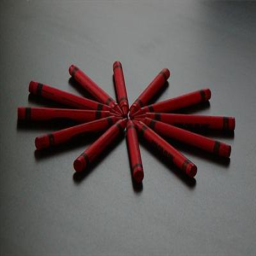
\includegraphics[width=0.25\textwidth]{example2.png}} 
  \subfigure[]{ 
    \label{fig: SDSPColorPrior: b} %% label for second subfigure 
    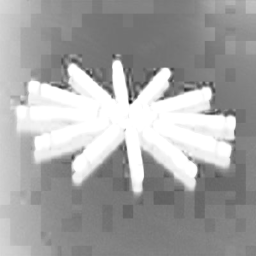
\includegraphics[width=0.25\textwidth]{SDSPColorPrior.png}} 
  \caption{SDSP: Color Prior}
  \label{fig: SDSPColorPrior} %% label for entire figure 
\end{figure}

%
% references
\bibliographystyle{plain}

\bibliography{features} %参考文献


\end{document}